
\documentclass{article}

\setlength{\parindent}{0pt}
\usepackage{cite}
\usepackage{enumerate}
\usepackage{tikz}
\usepackage{multirow}
\usepackage{longtable}
\newcommand\independent{\protect\mathpalette{\protect\independenT}{\perp}}
\def\independenT#1#2{\mathrel{\rlap{$#1#2$}\mkern2mu{#1#2}}}

\begin{document}

\title{Learning Causal Networks in Python}
\author{James Callan}
\date{}

\maketitle

\newpage


\section{Introduction}
The aim of this report is to detail the implementation of various algorithms to learn causal networks in python.These algorithms have already been implemented in the statistical programming environment R. However, recently python has become more widely used in the field of statistical computation.\\

Python offers a number of advantages over R. Python is much more widely used in general than R so an implementation in python would be accessible to a wider array of developers.Python is also used in a variety of settings as it is a general purpose programming language. This would allow the software implementation to be integrated into many different systems, written in python, with relative ease.\\

\section{Literature Review}

\subsection{Causal Networks}

Causal Networks are graphical models which represent a set of variables, their conditional dependencies, and their causal relationships\cite{verma1990causal} as a Directed Acyclic Graph (DAG) or a Maximal Ancestral Graph (MAG). The nodes of the Graph represent the variables. The edges of the graph represent causality, the direction of the edge represents the direction of causality with parent nodes causing child nodes\cite{verma1990causal}. 
\\

In a DAG all edges have a single direction, whereas in a MAG edges may be directed or bidirectional \cite{zhang2008causal}.
\\

\begin{center}
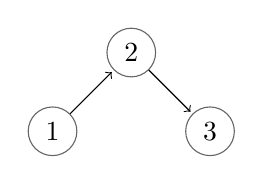
\begin{tikzpicture}[shorten >=1pt,->]
\tikzstyle{vertex}=[circle, draw=black!60, minimum size=12pt]
\node[vertex] (G_1) at (-1,-1) {1};
\node[vertex] (G_2) at (0,0)   {2};
\node[vertex] (G_3) at (1,-1)  {3};
\draw [->] (G_1) -- (G_2);
\draw [->] (G_2) -- (G_3);
\end{tikzpicture}
\end{center}

\begin{center}
Figure 1 A DAG with 3 nodes and 2 edges
\end{center}

\begin{center}
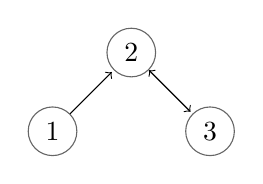
\begin{tikzpicture}[shorten >=1pt,->]
\tikzstyle{vertex}=[circle, draw=black!60, minimum size=12pt]
\node[vertex] (G_1) at (4,-1) {1};
\node[vertex] (G_2) at (5,0)   {2};
\node[vertex] (G_3) at (6,-1)  {3};
\draw [->] (G_1) -- (G_2);
\draw [<->] (G_2) -- (G_3);
\end{tikzpicture}\\
\end{center}

\begin{center}
Figure 2 A MAG with 3 nodes and 2 edges
\end{center}


The learning of causal networks allows relationships between variables to be uncovered and presented in a simple and human readable fashion. This can provide useful information for further data analysis as the set of variables that cause another could be used to predict it's value.
\\

\subsection{Probability and Independence}
In probability theory we can quantify our confidence in a particular event $ E $ occurring. This confidence, denoted as $ P(E) $ is a real number between 1 and 0. $  P(E) = 1 $ representing a certainty and $  P(E) = 0 $ representing $E$ being impossible.
\\

In the case of random variables an event would be a variable $X$ taking a particular value $x_i$, where $x_i$ is a member of the set $x = \{x_1, x_2, ..., x_n\}$ of possible values $X$ can take. The probability of this event is denoted as $P(X=x_i)$.
\\

The probability distribution $P(X=x)$ or simply $P(X)$ defines the probabilities for every value which $X$ can take. 
\\

Distributions of more than one variable can be described with joint distributions. For Variables $X$ and $Y$ the distribution $P(X,Y)$  describes the probability of both $X$ and $Y$ taking particular values simultaneously. 
\\

Joint distributions can also describe how the value of one variable can effect the value of an other. $P(X|Y)$ describes the probabilities of $X$ taking particular values ''given'' a value that $Y$ has taken. $P(X|Y)$ is defined as $P(X,Y)/P(Y)$.
\\

If two variables are independent there is no correlation between the values they take. That is for two variables $X$ and $Y$, the distribution $P(X|Y)$ would be the same for all values of $Y$. Therefore $P(X|Y) = P(X)$. If two variables are independent we can determine that there is no causal relationship between them.\\

Given the definition $P(X|Y) = P(X,Y)/P(Y)$ and $P(X|Y) = P(X)$ when $X$ and $Y$ are independent, it easy to see that $P(X,Y) = P(X)P(Y) $ if $X$ and $Y$ are independent.\\

Two variables $X$ and $Y$ can be considered independent conditioned on a third variable $Z$ if there is no correlation between $X$ and $Y$ for given the value of	 $Z$.\\

In this case $P(X|Y,Z) = P(X|Z)$, as the value of $Y$ has no impact on the value of $X$. The definition of conditional distributions shows $P(X|Y,Z) = \frac{P(X,Y,Z)}{P(Y,Z)}$, and $P(Y,Z) = P(Y|Z)P(Z)$. Using theses definitions and basic algebra $P(X,Y|Z) = P(X|Z)P(Y|Z)$ can be shown when $X$ and $Y$ are conditionally independent on $Z$.

\subsection{D Separation}

A path is any sequence of adjacent edges regardless of their directionality. A collider is node in a path which is both entered and left on edges which are directed toward the node. Unblocked refers to a path that does not traverse a collider\cite{pearl2003causality}.
\\
\begin{center}
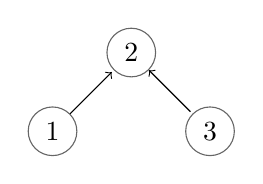
\begin{tikzpicture}[shorten >=1pt,->]
\tikzstyle{vertex}=[circle, draw=black!60, minimum size=12pt]
\node[vertex] (G_1) at (-1,-1) {1};
\node[vertex] (G_2) at (0,0)   {2};
\node[vertex] (G_3) at (1,-1)  {3};
\draw [->] (G_1) -- (G_2);
\draw [<-] (G_2) -- (G_3);
\end{tikzpicture}
\end{center}

\begin{center}
Figure 3 A graph containing a collider
\end{center}

If every path between nodes $ X $ and $ Y $ traverses a collider, nodes $ X $ and $ Y $ are unconditionally d-separated or d-separated conditioned on the empty set \cite{pearl2003causality}. Two unconditionally d-separated nodes in a causal network are considered to be independent\cite{pearl2009}.
\\
\begin{center}
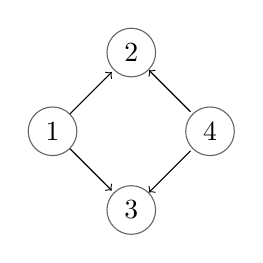
\begin{tikzpicture}[shorten >=1pt,->]
\tikzstyle{vertex}=[circle, draw=black!60, minimum size=12pt]
\node[vertex] (G_1) at (-1,-1) {1};
\node[vertex] (G_2) at (0,0)   {2};
\node[vertex] (G_3) at (0,-2)  {3};
\node[vertex] (G_4) at (1,-1)  {4};
\draw [->] (G_1) -- (G_2);
\draw [<-] (G_2) -- (G_4);
\draw [->] (G_1) -- (G_3);
\draw [<-] (G_3) -- (G_4);
\end{tikzpicture}
\end{center}

\begin{center}
Figure 4
\end{center}

\begin{center}
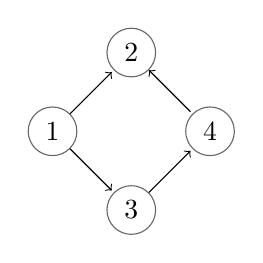
\begin{tikzpicture}[shorten >=1pt,->]
\tikzstyle{vertex}=[circle, draw=black!60, minimum size=12pt]
\node[vertex] (G_1) at (4,-1) {1};
\node[vertex] (G_2) at (5,0)   {2};
\node[vertex] (G_3) at (5,-2)  {3};
\node[vertex] (G_4) at (6,-1)  {4};
\draw [->] (G_1) -- (G_2);
\draw [<-] (G_2) -- (G_4);
\draw [->] (G_1) -- (G_3);
\draw [->] (G_3) -- (G_4);
\end{tikzpicture}
\end{center}

\begin{center}
Figure 5
\end{center}


Two nodes X and Y are d-separated conditioned on set Z if:
\begin{enumerate}
	\item There exists no unblocked path from $ X $ to $ Y $ that does not traverse any members of $ Z $.\cite{pearl2003causality}
	\item There is no blocked path from $ X $ to Y in which all colliders are members of $ Z $ or have descendants in $ Z $. \cite{pearl2003causality}
\end{enumerate} 

Causal networks represent conditional independence with d-separation, variables X and Y are conditionally independent on set Z if nodes X and Y are d-separated conditioned on nodes in set Z\cite{verma1990causal}.
\\

\subsection{Faithfulness}


By testing for d-separation of variables X and Y given conditioning set Z on a graph we can see if $X \independent Y | Z$ \cite{pearl2009}. However, the reverse is only true if the distribution is faithful to the graph. That is, if a distribution is faithful to a graph then all independence relationships are represented on the graph and only these relationships are present \cite{scheines1997introduction}. Assuming faithfulness allows the topology of a graph to be learned by testing pairs of variables for independence given various conditioning sets.
\\

\subsection{Discriminating paths}
For the FCI and RFCI algorithms the notion of discriminating paths is needed. A path $\pi$ = (A, .., X,Y,Z) is discriminating a discriminating path for Y if:
\\

\begin{enumerate}
\item $\pi$ must include at least 3 edges
\item Y is a non-endpoint on $\pi$ and is adjacent to Z on $\pi$.
\item A is not adjacent to Z and every other node is a collider on $\pi$ and a parent of Z. \cite{colombo2012learning} 
\end{enumerate}

\begin{center}
	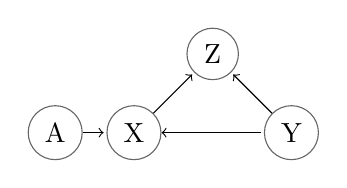
\begin{tikzpicture}[shorten >=1pt,->]
	\tikzstyle{vertex}=[circle, draw=black!60, minimum size=12pt]
	\node[vertex] (G_1) at (0,0) {A};
	\node[vertex] (G_2) at (1,0)   {X};
	\node[vertex] (G_3) at (3,0)  {Y};
	\node[vertex] (G_4) at (2,1)  {Z};
	\draw [->] (G_1) -- (G_2);
	\draw [<-] (G_2) -- (G_3);
	\draw [->] (G_2) -- (G_4);
	\draw [->] (G_3) -- (G_4);
	\end{tikzpicture}
\end{center}

\begin{center}
	Figure 6 \\
	(A,X,Y,Z) is a discriminating path on Y
\end{center}

\subsection{Tests for Independence}
When trying to find causal relations between variables tests for independence and conditional independence must be performed. These tests allow us to find correlation between variables and also find out if the correlation between two variables is actually caused by another.\\

One such test is the $\chi^2$ test, this test gives the probability that some data was drawn from a particular distribution.\\

If the variables $X$ and $Y$ are independent then $p(X,Y) = p(X)p(Y)$. Both of these distributions can be calculated from data. The $\chi^2$ test can then be used to find the probability that they are equal.\\

To estimate $p(X,Y)$ the counts of all pairs of values taken by the variables can be found. They can then divided by the count of all data points. These counts can be stored in a table with the values of $X$ as columns, values of $Y$ as rows (or visa versa) and entries as observed counts, for ease of access. This type of table is known as a contingency table.\\

\begin{table}[h!]
	\centering
	\begin{tabular}{c|c}
		X & Y \\ \cline{1-2}
		1 & 0 \\
		1 & 1 \\ 
		0 & 1 \\ 
		1 & 1 \\ 
		0 & 0 \\ 
		1 & 1 \\ 
		1 & 0 \\ 
	\end{tabular}
	\begin{tabular}{c|c|cc|}
		\multicolumn{2}{c}{}& \multicolumn{2}{c}{X} \\ \cline{3-4}
		\multicolumn{2}{c|}{} & 0 & 1 \\ \cline{2-4}
		\multirow{2}{*}{Y} & 0 & 1 & 2\\
		& 1 & 1 & 3 \\
		\cline{2-4} 
	\end{tabular}
\end{table}

To estimate the distribution $p(X)$, the count of points in which $X$ takes a value over the total number of points for all values of $X$. The counts can be found with the sum of the columns of the contingency table. The same can be done for $p(Y)$ with the rows of the table.\\

The $\chi^2$ statistic can then be calculated with:

\begin{center}
	$\chi^2 = \sum\frac{(p(X)p(Y)-p(X,Y))^2}{p(X)p(Y)}$
\end{center}

The $\chi^2$ value can then be passed to a cumulative density function and a p-value returned. The function used is dependent upon the degrees of freedom. The degrees of freedom are equal to the $(no. rows -1)*(no. columns -1)$. The p-value represents how likely it is that the two variables are independent.\\

The test is similar for conditional independence. The $chi^2$ statistic now depends on conditional distributions. If $X \independent Y | Z$ $p(X,Y|Z) = p(X|Z)p(Y|Z)$. Therefore:\\

\begin{center}
	$\chi^2 = \sum\frac{(p(X|Z)p(Y|Z)-p(X,Y|Z))^2}{p(X|Z)p(Y|Z)}$
\end{center}

These values can all be found by calculating a contingency table for $X,Y and Z$.\\

This statistic can then be used in the same way as before to calculate a p-value. However, the degrees of freedom are multiplied by the possible values of Z -1. 

\subsection{Algorithms For Learning Causal Networks}
\subsubsection{Constraint Based Methods}
 There have been a number of algorithms developed to learn graphical causal representations from data. Over the course of this project, I plan to implement: The PC algorithm \cite{spirtes1991algorithm}, the Fast Causal Inference (FCI) algorithm \cite{colombo2012learning}, and the Really Fast Causal Inference (RFCI) Algorithm \cite{colombo2012learning}.
\\

Rather than learning an individual DAG the PC algorithm learns a set of DAGs which could represent the causal relationships found in the data. In cases where the direction of an edge is unclear no direction is specified. The output of the algorithm is a partially directed acyclic graph which represents the set DAGs with all possible orientations of undirected edges\cite{spirtes1991algorithm}.
\\

The FCI and RFCI algorithms learn partial ancestral graphs (PAGs) which represent the set of MAGs that fit the data \cite{colombo2012learning}. Unlike in the PC algorithm if the direction of an edge can not be determined it is assumed that there is some set of latent variables influencing the nodes being tested. Each end of an edge can be one of three things in a PAG, an arrow in every MAG ($>$), a tail in every MAG ($-$) or an arrow in at least one MAG and a tail in at least one MAG ($o$), ends of an edge denoted by $*$ can be any of the specified types. This allows for a richer display of information than a partial DAG\cite{colombo2012learning}.
\\

The PAG generated by the FCI algorithm is considered to be less accurate than the PAG generated by the RFCI algorithm. This is because the FCI algorithm performs more tests than the RFCI algorithm. These tests give us more confidence in the presence and the orientation of edges however this comes at the cost of speed.
\\
\subsubsection{Score Based Methods}
The above algorithms are all constraint based. There is another class of algorithm which are score based. Rather than finding graphs using the rules that define the networks, score based methods generate random graphs and assign them a score based on how well they fit data.\\

   
\subsection{Computing a skeleton}
All three algorithms begin by calculating the skeleton of the graph. The skeleton consists of the edges that are present in the partial DAG or PAG however all edges are undirected. The separation set of two variables ($sepSet(x,y)$) contains the smallest set of variables that the pair are conditionally independent on.  When calculating the skeleton the separation set of each pair of variables is also recorded as it is needed to orient the edges of the graph\cite{colombo2012learning, spirtes1991algorithm}.
\\

The skeleton is calculated using a series of conditional independence tests. These conditional independence tests are dependent on the type of input data, therefore conditional independence tests can be defined independently of the algorithm. The conditional independence tests must be able to determine if two variables are indpendent based on some set of other variables from data.
\\

To begin the skeleton computation the fully connected undirected graph of all variables is constructed and then conditional independence tests are performed to determine which edges to remove.
\\

Adjacent pairs of variables are tested for independence conditioned upon set of variables adjacent to them. The size of these sets starts at 0 but is incremented after all adjacent pairs have been tested. This repeats until there are not enough adjacent variables to fill the conditioning set.\\

 The edges which have not been removed form the skeleton of the graph which is needed for the PC, FCI and RFCI algorithms along with the recorded separation sets of removed edges \cite{colombo2012learning, spirtes1991algorithm}.
\\

\begin{table}[h!]
	\begin{tabular}{|l l|}
		 \hline
		 \multicolumn{2}{|l|}{Algorithm to Estimate Skeleton}\\ 
		 \hline
		 \textbf{Input}: & Data, Independence Test\\
		 \textbf{Output}: & Estimated Skeleton, Separation Sets of Variables\\
		 &\\
		 \multicolumn{2}{|l|}{k = 0}\\
		 \multicolumn{2}{|l|}{N = list of variables in data}\\
		 \multicolumn{2}{|l|}{G = fully connected undirected graph with nodes = N}\\
		 &\\
		 \multicolumn{2}{|l|}{\textbf{while} there is some S $\in $ adj(X, G) $\setminus$ Y \textbf{where} $ | $S$ | $ = k \textbf{for} some X \textbf{in} N \textbf{and} Y \textbf{in} adj(X,G)}\\
		 \multicolumn{2}{|l|}{\quad\textbf{for all} X \textbf{in} N:}\\
		 \multicolumn{2}{|l|}{\quad\quad \textbf{for all} Y \textbf{in} adj(X, G):}\\
		 \multicolumn{2}{|l|}{\quad\quad\quad \textbf{for all} S $\in $ adj(X, G) $\setminus$ Y \textbf{where} $ | $S$ | $ = k:}\\
		 \multicolumn{2}{|l|}{\quad \quad \quad\quad \textbf{if} X $ \independent $ Y $ | $ S}\\
		 \multicolumn{2}{|l|}{\quad \quad \quad \quad\quad remove edge X,Y from G}\\
		 \multicolumn{2}{|l|}{\quad \quad \quad \quad\quad sepSet(X,Y) = S}\\
		 \multicolumn{2}{|l|}{\quad \quad \quad \quad\quad break}\\
		 \multicolumn{2}{|l|}{\quad \quad \quad\quad \textbf{end if}} \\
		 \multicolumn{2}{|l|}{\quad \quad\quad \textbf{end for}}\\
		 \multicolumn{2}{|l|}{\quad\quad \textbf{end for}}\\
		 \multicolumn{2}{|l|}{\quad\textbf{end for}}\\
		 \multicolumn{2}{|l|}{\quad k += 1}\\
		 \multicolumn{2}{|l|}{ \textbf{end while}}\\
		 &\\
		 \multicolumn{2}{|l|}{ \textbf{return} G, sepSet}\\
		 \hline
		 
	\end{tabular}
\end{table}
\subsection{The PC Algorithm}
After generating the skeleton and separation sets of pairs of nodes, the pc algorithm attempts to orient the undirected edges of the graph.
\\

It begins by searching for colliders. For each triple of vertices A, B, and C where A and B are adjacent, B and C are adjacent, but A and C are not adjacent orient the edges A-B-C to A$\rightarrow$B$\leftarrow$C if B is not in the separation set of the pair (A,C).
\\

Once colliders are specified other edges can be oriented. This is done by repeating two steps until no more edges can be given a direction. The algorithm for edge orientation is described in.\\
\\

\begin{table}[h!]
	\begin{tabular}{|l l|}
		\hline
		\multicolumn{2}{|l|}{PC Algorithm to Orient Edges}\\ 
		\hline
		\textbf{Input}: & Skeleton of Causal Network, Separation sets of variables\\
		\textbf{Output}: & Partial Directed Acyclic Graph\\
		&\\
		\multicolumn{2}{|l|}{G = Skeleton of network}\\
		\multicolumn{2}{|l|}{N = nodes of G}\\
		&\\
		\multicolumn{2}{|l|}{\textbf{for all} $ i,j,k $ in N:}\\
		\multicolumn{2}{|l|}{\quad\textbf{if} $ k $ \textbf{not in} $ adj(i,G) $ \textbf{and} $ j $ \textbf{in} $sepSet( i,k)$:}\\
		\multicolumn{2}{|l|}{\quad\quad orient $ i-j-k $ as $ i\rightarrow j \leftarrow k $ }\\
		\multicolumn{2}{|l|}{\quad\textbf{end if}}\\
		\multicolumn{2}{|l|}{\textbf{end for}}\\
		&\\
		\multicolumn{2}{|l|}{\textbf{while} no more edges can be oriented:}\\
		\multicolumn{2}{|l|}{\quad\textbf{for all} $ i,j,k $ in N:}\\
		\multicolumn{2}{|l|}{\quad\quad\textbf{if} $ k $ \textbf{not in} $ adj(i,G) $:}\\
		\multicolumn{2}{|l|}{\quad\quad\quad orient $ i\rightarrow j-k $ as $ i\rightarrow j \rightarrow k $ }\\
		\multicolumn{2}{|l|}{\quad\quad\textbf{end if}}\\
		\multicolumn{2}{|l|}{\quad\quad\textbf{if} $ directedpath(i,j)$ \textbf{in} $G $:}\\
		\multicolumn{2}{|l|}{\quad\quad\quad orient $ i- j $ as $ i\rightarrow j $ }\\
		\multicolumn{2}{|l|}{\quad\quad\textbf{end if}}\\

		\multicolumn{2}{|l|}{\quad\textbf{end for}}\\
		\multicolumn{2}{|l|}{\textbf{end while}}\\
		&\\
		\multicolumn{2}{|l|}{\textbf{return} G}\\
		\hline 
	\end{tabular}
\end{table}



\subsection{The FCI algorithm}

The FCI algorithm starts in the same way as the PC algorithm using exactly the process of conditional independence tests to estimate a skeleton of the final graph. It also orients colliders in the same way, producing a PDAG.
\\

Next, the final skeleton of the graph is obtained from the PDAG G. To do this The possible d-separators of every variable must be found in G. For variable X, the possible d separators set in nG ($PossibleDSep(X,G)$) consists of all variables Y for which there is some path $\pi = path(X,Y)$ in G, such that in every sub path $A,B,C$, $B$ is a collider or $A,B,C$ form a triangle. All adjacent variables ($X,Y$) are the tested for conditional independence, conditioned on every subset of each of the possible d separators set. If the test finds conditional independence the edge $X,Y$ is removed and the conditioning set recorded as a separation set. 
\\

The PDAG can then be converted to a PAG by setting all edges to $o-o$.\\

Next the colliders must be reoriented. This is done on a similar way however now edges can be bi-directional.\\

Once the final skeleton has been estimated, A series of orientation rules can be performed repeatedly until no more orientations can be found. Theses rules are described in.\\


	\begin{longtable}{|l l|}
		\hline
		\multicolumn{2}{|l|}{FCI Algorithm to Orient Edges}\\ 
		\hline
		\textbf{Input}: & Skeleton of Causal Network, Separation sets of variables\\
		\textbf{Output}: & Partial Ancestral Graph\\
		&\\
		\multicolumn{2}{|l|}{G = Skeleton of network}\\
		\multicolumn{2}{|l|}{N = nodes of G}\\
		&\\
		\multicolumn{2}{|l|}{\textbf{for all} $ i,j,k $ in N:}\\
		\multicolumn{2}{|l|}{\quad\textbf{if} $ k $ \textbf{not in} $ adj(i,G) $ \textbf{and} $ j $ \textbf{in} $sepSet( i,k)$:}\\
		\multicolumn{2}{|l|}{\quad\quad orient $ i-j-k $ as $ i\rightarrow j \leftarrow k $ }\\
		\multicolumn{2}{|l|}{\quad\textbf{end if}}\\
		\multicolumn{2}{|l|}{\textbf{end for}}\\
		&\\
		
		\multicolumn{2}{|l|}{\textbf{for all} i in N and j in adj(i,G):}\\
		\multicolumn{2}{|l|}{\quad \textbf{for all} $T \subseteq PossibleDSep(i,G)\setminus \{i,j\}$:}\\
		\multicolumn{2}{|l|}{\quad\quad \textbf{if} $i \independent j | T$:}\\
		\multicolumn{2}{|l|}{\quad\quad \quad remove edge i,j from G}\\
		\multicolumn{2}{|l|}{\quad\quad \quad $sepSet(i,j) = T$}\\	
		\multicolumn{2}{|l|}{\quad\quad \quad $sepSet(j,i) = T$}\\
		\multicolumn{2}{|l|}{\quad\quad \quad break}\\
		\multicolumn{2}{|l|}{\quad\quad\textbf{end if}}\\
		\multicolumn{2}{|l|}{\quad\textbf{end for}}\\
		\multicolumn{2}{|l|}{\quad \textbf{for all} $T \subseteq PossibleDSep(j,G)\setminus \{i,j\}$:}\\
		\multicolumn{2}{|l|}{\quad\quad \textbf{if} $i \independent j | T$:}\\
		\multicolumn{2}{|l|}{\quad\quad \quad remove edge i,j from G}\\
		\multicolumn{2}{|l|}{\quad\quad \quad $sepSet(i,j) = T$}\\	
		\multicolumn{2}{|l|}{\quad\quad \quad $sepSet(j,i) = T$}\\
		\multicolumn{2}{|l|}{\quad\quad \quad break}\\
		\multicolumn{2}{|l|}{\quad\quad\textbf{end if}}\\
		\multicolumn{2}{|l|}{\quad\textbf{end for}}\\
		\multicolumn{2}{|l|}{\textbf{end for}}\\	
		&\\
		
		\multicolumn{2}{|l|}{set all edges in G to o-o}\\
		&\\
		\multicolumn{2}{|l|}{\textbf{for all} $ i,j,k $ in N:}\\
		\multicolumn{2}{|l|}{\quad\textbf{if} $ k $ \textbf{not in} $ adj(i,G) $ \textbf{and} $ j $ \textbf{in} $sepSet( i,k)$:}\\
		\multicolumn{2}{|l|}{\quad\quad orient $ i*-*j*-*k $ as $ i*\rightarrow j \leftarrow *k $ }\\
		\multicolumn{2}{|l|}{\quad\textbf{end if}}\\
		\multicolumn{2}{|l|}{\textbf{end for}}\\
		&\\
		
		\multicolumn{2}{|l|}{\textbf{while} no more edges can be oriented:}\\
		\multicolumn{2}{|l|}{\quad\textbf{for all} $ i,j,k,l $ in N:}\\
		\multicolumn{2}{|l|}{\quad\quad\textbf{if} $ directedpath(i,j)$ \textbf{in} $G $:}\\
		\multicolumn{2}{|l|}{\quad\quad\quad orient $ i*-*j $ as $ i*\rightarrow j $ }\\
		
		\multicolumn{2}{|l|}{\quad\quad\textbf{else if} $i*\rightarrow j *-* k$ in G: }\\
		
		\multicolumn{2}{|l|}{\quad\quad\quad orient $i*\rightarrow j *-* k$ as $i*\rightarrow j \rightarrow k$}\\
		
		\multicolumn{2}{|l|}{\quad\quad\textbf{else if} $i*\rightarrow j \leftarrow * k$ in G \textbf{and} $l \in adj(j,G)$ \textbf{and} $k \notin adj(i)$: }\\
		
		\multicolumn{2}{|l|}{\quad\quad\quad orient $j *-* l$ as $j \leftarrow *l$}\\
		
		\multicolumn{2}{|l|}{\quad\quad\textbf{else if} $i\leftarrow* j$ \textbf{in} G \textbf{and} $i\rightarrow k$ \textbf{in} G \textbf{and} $k o-* j$ \textbf{in} G: }\\
		
		\multicolumn{2}{|l|}{\quad\quad\quad orient $k o-* j$ as $k \leftarrow* j$}\\
		
		\multicolumn{2}{|l|}{\quad\quad\textbf{else if} $l \in adj(j,DiscPath(i,j,k))$ \textbf{and} i,l,k form a triangle in G:}\\
		
		\multicolumn{2}{|l|}{\quad\quad\quad \textbf{if} $k \notin sepset(i,j)$:}\\
		
		\multicolumn{2}{|l|}{\quad\quad\quad\quad orient $l *-* k *-*j$ as $l *\rightarrow k \leftarrow * j$}\\
		
		\multicolumn{2}{|l|}{\quad\quad\quad \textbf{else}: }\\
		\multicolumn{2}{|l|}{\quad\quad\quad\quad mark $k$ as non-collider on path $(l,k,j)$ }\\
		\multicolumn{2}{|l|}{\quad\quad\quad \textbf{end if}: }\\
		\multicolumn{2}{|l|}{\quad\quad \textbf{end if}: }\\
		\multicolumn{2}{|l|}{\quad\textbf{end for}}\\
		\multicolumn{2}{|l|}{\textbf{end while}}\\
		&\\
		\multicolumn{2}{|l|}{\textbf{return} G}\\
		\hline 
	\end{longtable}

\subsection{RFCI Algorithm}
Like the other two algorithms the RFCI begins by estimating the skeleton of the final graph.
\\

Next the colliders in the graph are found, this is done differently than in the two previous algorithms. We created and empty list L and for each triple (A,B,C) in the list of unshielded triples we check if both:
\\

\begin{enumerate}[i]
	\item $A \independent$ $B$ $|$ $((sepset(A,B) \setminus \{C\}))$
	\item $B \independent$ $C$ $|$ $((sepset(A,B) \setminus \{C\}))$\end{enumerate}
where sepset(X,Y) is the separating set of Nodes X and Y. If both of these tests hold, add to list L. If only the first test holds, find the minimal separating set of A and B and record it as the separating set of A and B. Next, remove the edge A-B, add any newly create unshielded triples to M, and remove any destroyed triples from L and M. If only the second test passes do the same as above but for nodes B and C.
\\

Finally the edges must be oriented. To begin edge orientation apply rules $R1-R3$ found in \cite{ZHANG20081873}. Next triangles (X,Y,Z) must be found with edges $Yo-*Z$, $X<-*Y$, and $X-->Z$. Once a triangle is found the shortest discriminating path from X to Z must be found.
\\

If a path $\pi$ exists take each pair of adjacent variables A and B on $\pi$ and creator a counter $l = 0$. Next find  a subset Y  $\subseteq (sepset(X,Y) \setminus \{A,B\})$ where $|Y| = l$. Then if $A \independent B | Y \cup S$ let sepset(A,B) = Y, delete the edge $A*-*B$ from the graph and update newly formed unshielded triples orientation using the collider orientation described earlier. If the conditional independence test fails increment $l$ and try again, testing with all subsets Y of size $l$, repeat this process until no set Y exists where |Y| = $l$ or the edge $A*-*B$ is removed. 
\\

If no edges are removed from $\pi$ by the above process then either: orient $Yo-*Z$ as $Y-->Z$ if Y is in the sperating set of X and Z or orient $X<-*Yo-*Z$ as $X<->Y<->Z$ if not.
\\

Finally orient as many edges using rules $R5-R10$ from \cite{ZHANG20081873}.
\\

This whole process must be repeated until it no longer alters any orientations.\cite{colombo2012learning}

\bibliography{Report}{}
\bibliographystyle{unsrt}
\end{document}